%Appenndix for line measurements in IRTF + other spectra

%\label{app:line_measure}

\chapter{Appendix}
\label{app:my_appendix}

\lhead{\emph{Appendix}}

%%%%%%%%%%%%%%%%% APPENDICES %%%%%%%%%%%%%%%%%%%%%


\subsection{Ephemeris data}
\label{sect:ephemeris data}

ASASSN-16kr has existing ephemeris data in the literature \citep{kato2017}, whereas SSSJ0522-3505 and ASASSN-17jf were reported with tentative period estimates. These were used as starting points, and eclipse times from this work were used to refine the $T_\mathrm{0}$\ and $P$\ for all three systems. Only ULTRACAM eclipse timings were used to calculate the ephemerides in this paper.

To calculate the time of white dwarf mid-eclipse for each observation, the numerical derivative of the flux was fit with a a double-Gaussian model, as described in \citet{wood1985}.
Ideally, the derivative shows a negative peak at white dwarf ingress, and a symmetrical positive peak at egress, and each would be equidistant from the white dwarf mid-eclipse time, $T_\mathrm{ecl}$. By fitting the double-Gaussian model to a smoothed, numerical derivative of the lightcurve using a Markov Chain Monte Carlo (MCMC) method using a Gaussian process to evaluate the log-likelihood, we obtain $T_\mathrm{ecl}$ with uncertainties for each eclipse.

For each observed $T_\mathrm{ecl}$, its eclipse number $N$\ (the number of eclipses since $T_0$) could unambiguously be determined from prior ephemeris data. 
An MCMC algorithm was used to fit a straight line model to the independent variable $N$\ and dependent variable $T_\mathrm{ecl}$, with a gradient $P$\ and intercept $T_0$. The model accounts for potential systematic differences in timing accuracy between instruments by also having variable error scale factors applied to all eclipses observed with a specific instrument, e.g. the timing reported for eclipses observed with ULTRACAM may be systematically offset from reality, and the errors associated with those observations might need to be larger than reported to be consistent with data from other instruments. The prior distribution assumed for these error factors was log-uniform ranging from 0.01 to 100, which favours the smallest factor consistent with the data. The values of $N$ for each system were chosen to minimise the covariance between $T_0$ and $P$.


\clearpage
\onecolumn
\section{Lightcurves}
\label{appendix:lightcurves}

\begin{figure}
    \centering
    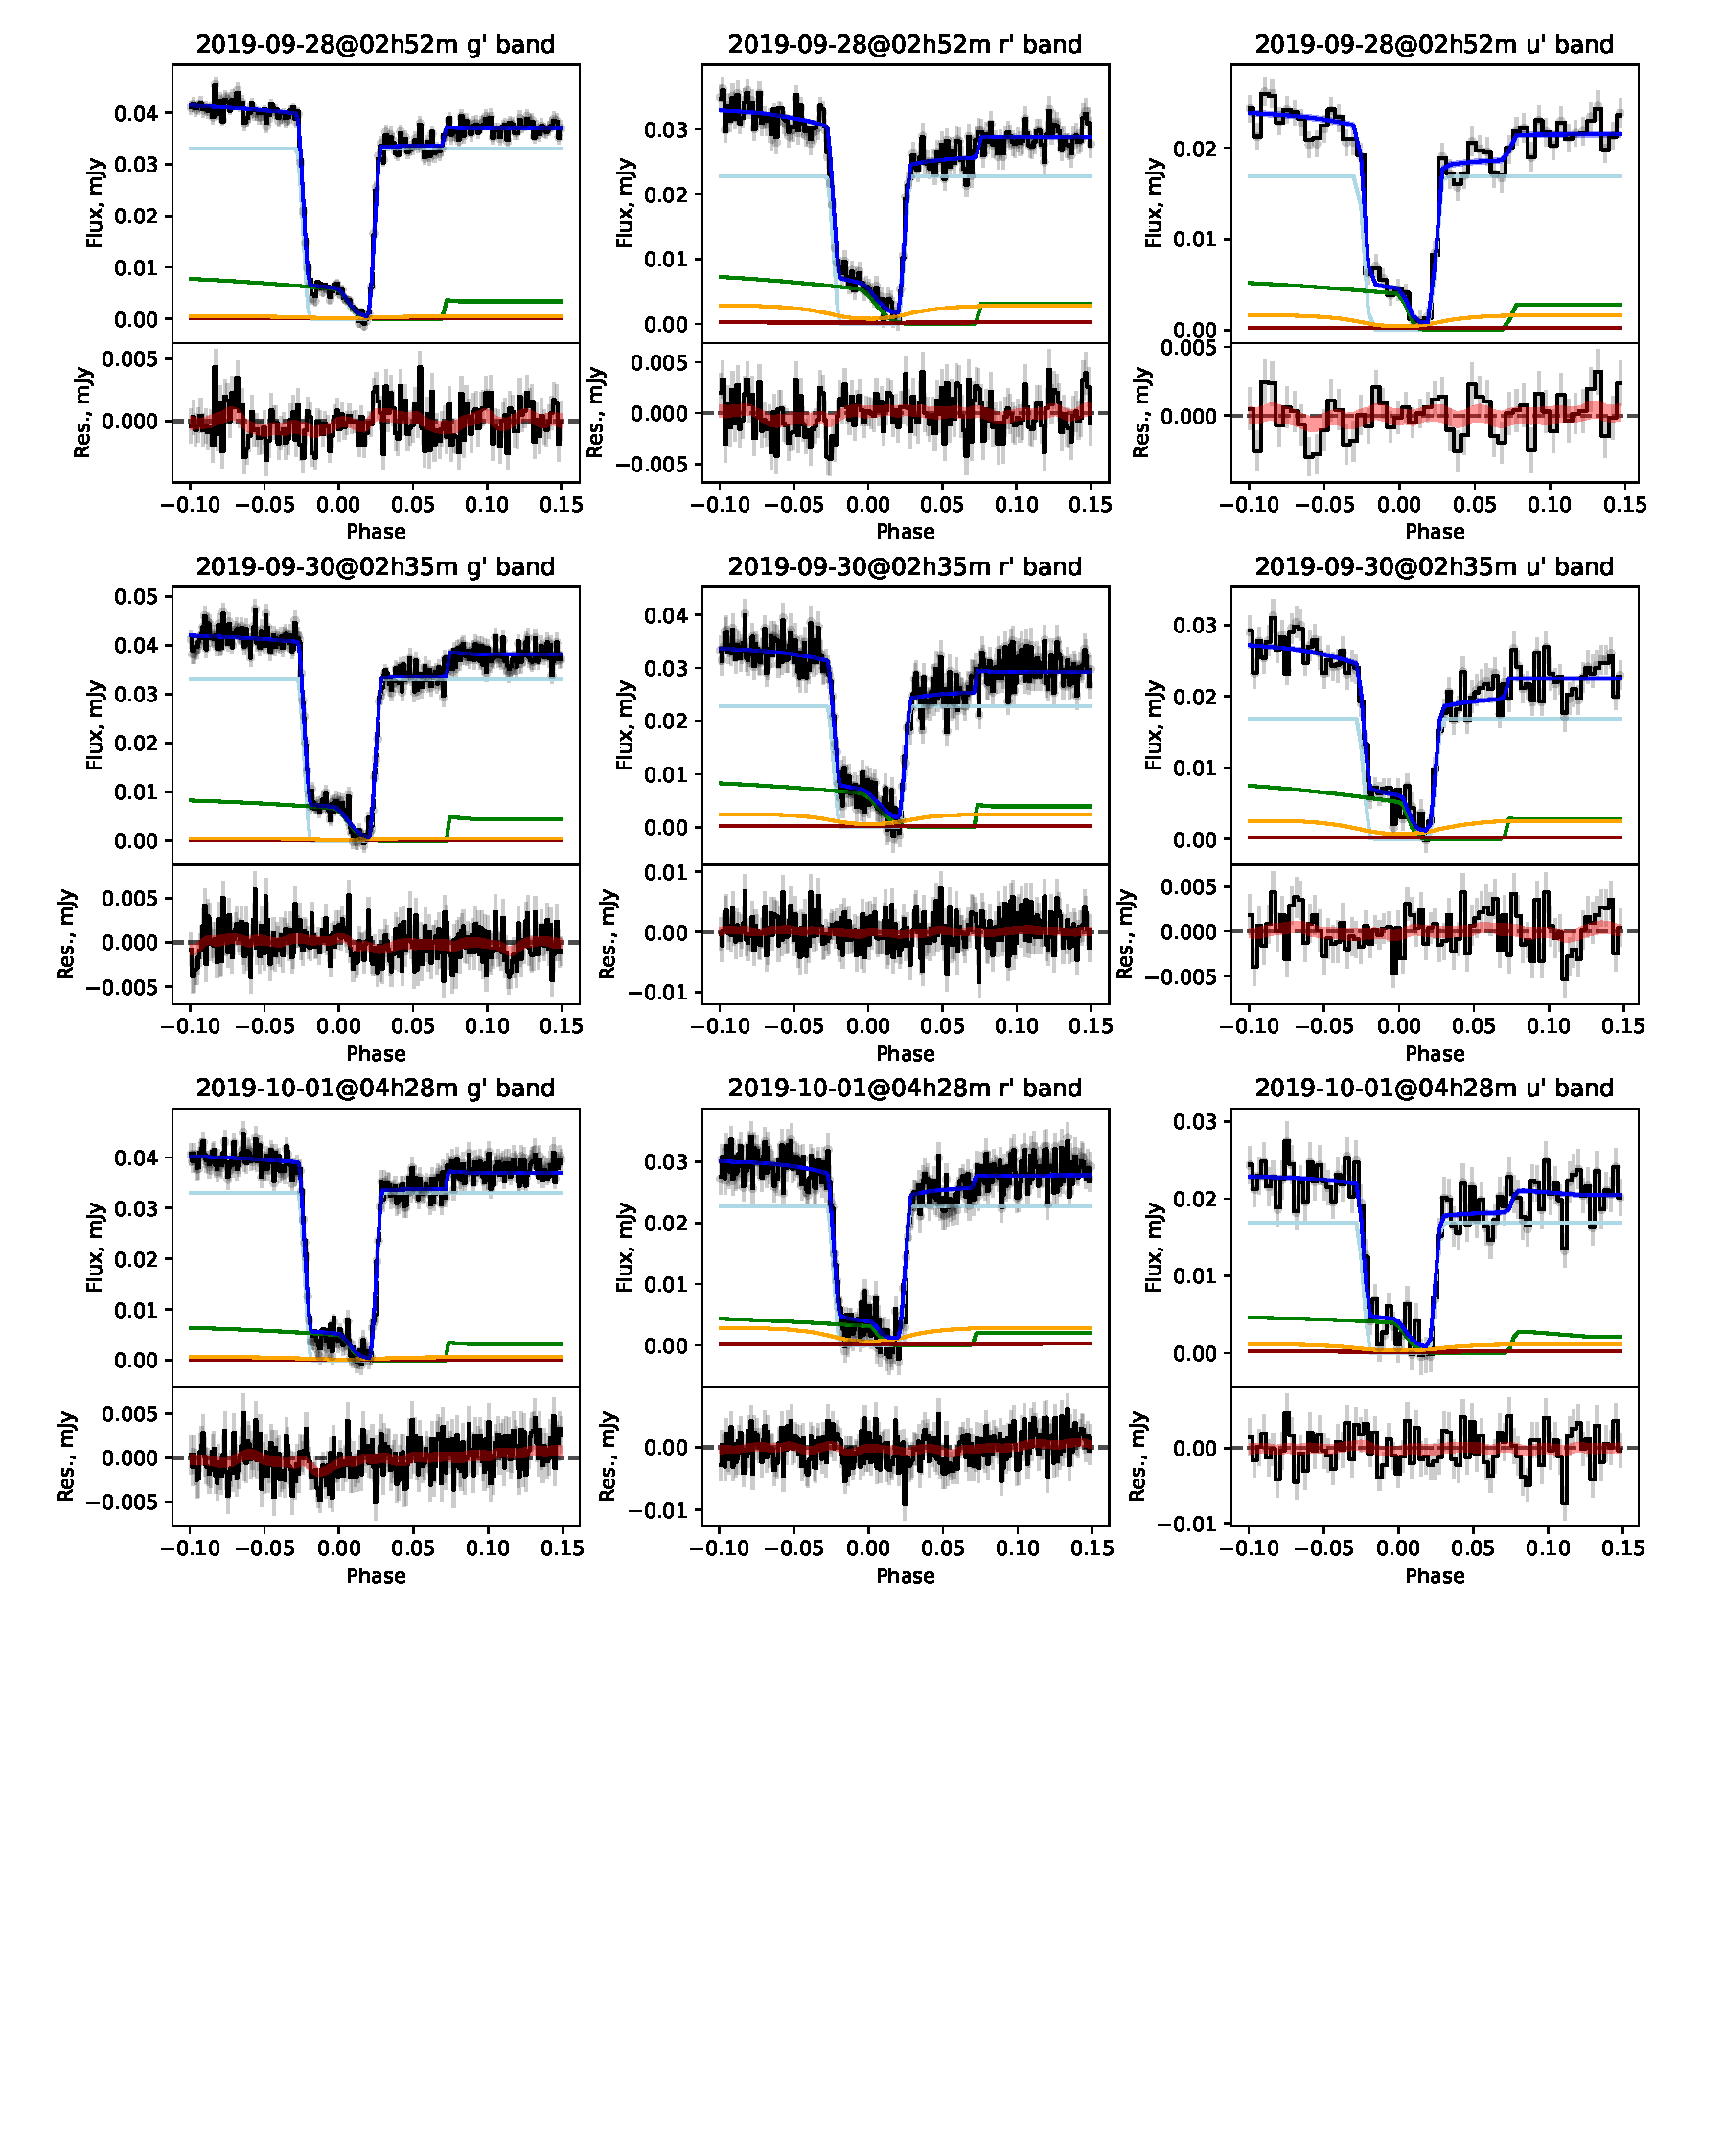
\includegraphics[width=\columnwidth, trim={0 10cm 0 0}, clip]{figures/three_cvs_with_weird_colours/ASASSN-17jf/ASASSN-17jf_lightcurves_3.pdf}
    \caption{ASASSN-17jf lightcurve models. {\it Top}:~grey points are the observed flux; black line is the observed flux, with the mean Gaussian process sample subtracted; the dark blue line is the mean lightcurve model, and the blue band is the standard deviation on this in the MCMC chain. The components of the model are also shown: the light blue line is the white dwarf flux, green line is the bright spot, orange line is the disc, and the red line is the donor. {\it Bottom}:~The residuals between the data and model are plotted as the black line, with grey error bars. The Gaussian process 1-sigma region is shown as a red band.}
    \label{fig:ASASSN-17jf all lightcurves}
\end{figure}

\begin{figure}
    \centering
    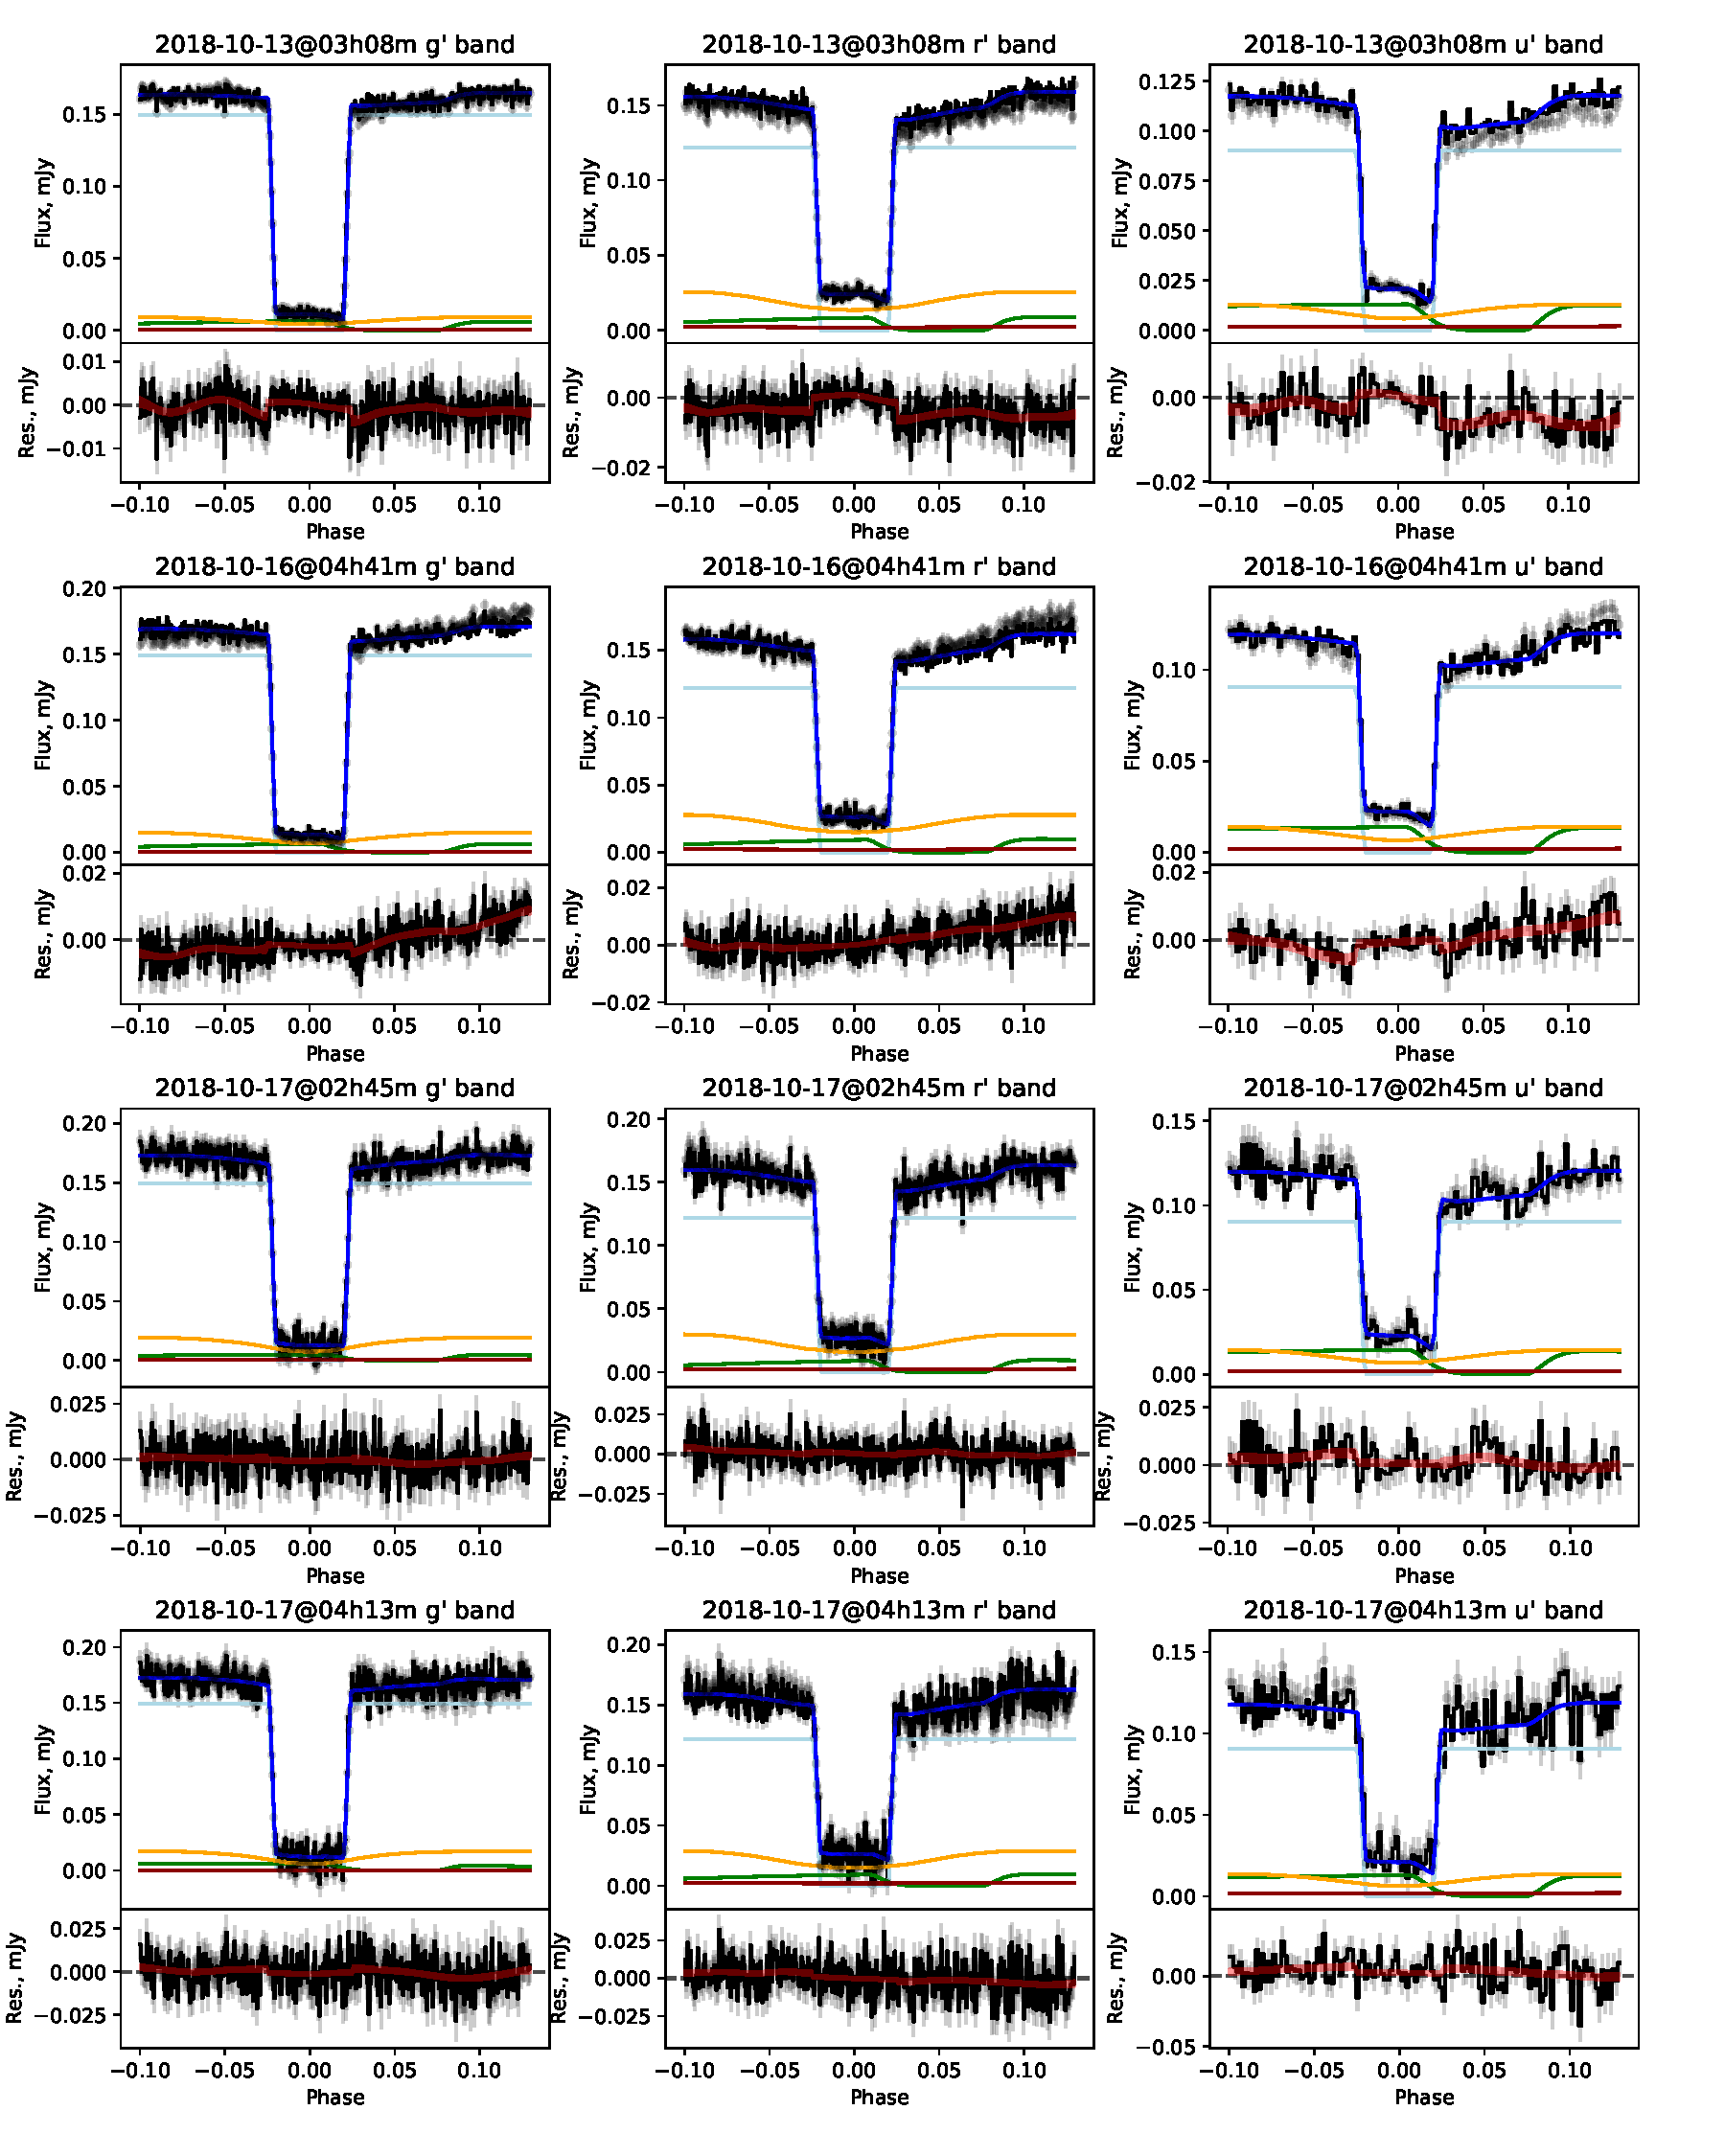
\includegraphics[width=\columnwidth, trim={0 0cm 0 0}, clip]{figures/three_cvs_with_weird_colours/ASASSN-16kr/ASASSN-16kr_lightcurves_3.pdf}
    \caption{ASASSN-16kr lightcurve models. Symbols are the same as Figure \ref{fig:ASASSN-17jf all lightcurves}}
    \label{fig:ASASSN-16kr all lightcurves}
\end{figure}
\begin{figure}
    \centering
    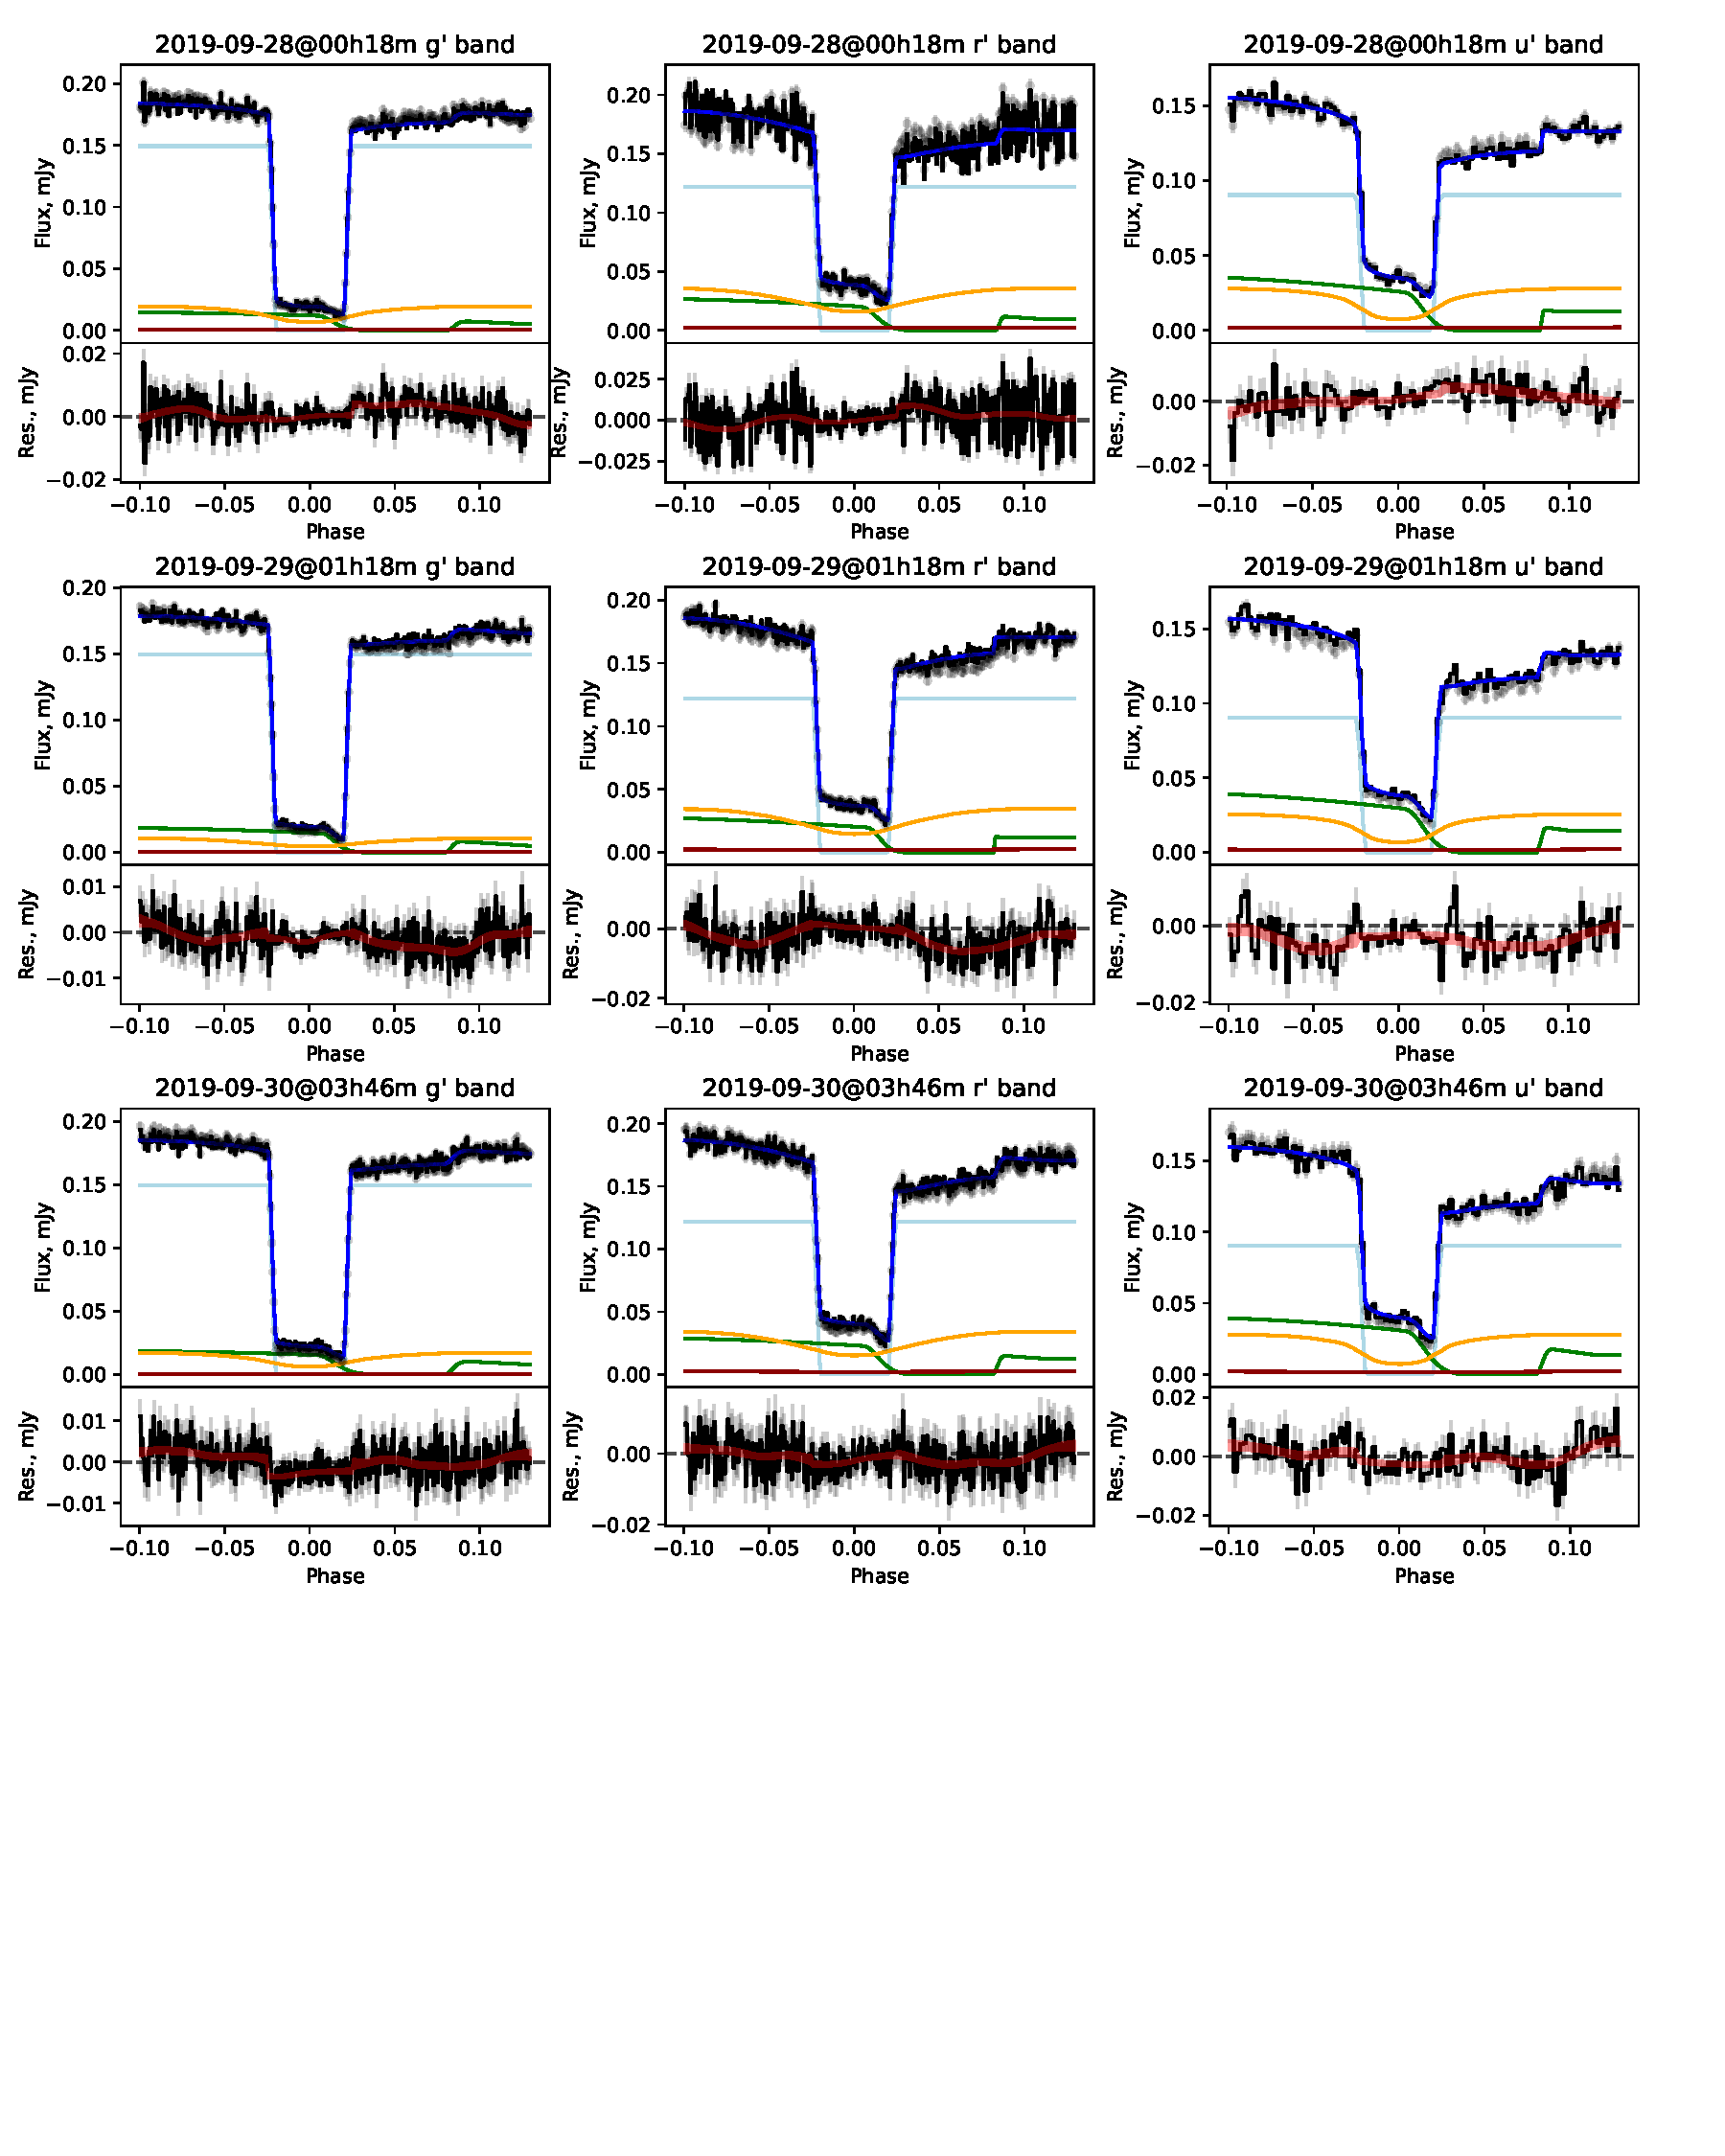
\includegraphics[width=\columnwidth, trim={0 10cm 0 0}, clip]{figures/three_cvs_with_weird_colours/ASASSN-16kr/ASASSN-16kr_lightcurves_6.pdf}
    \caption{ASASSN-16kr lightcurve models (cont.)}
    \label{fig:ASASSN-16kr all lightcurves cont}
\end{figure}


\begin{figure}
    \centering
    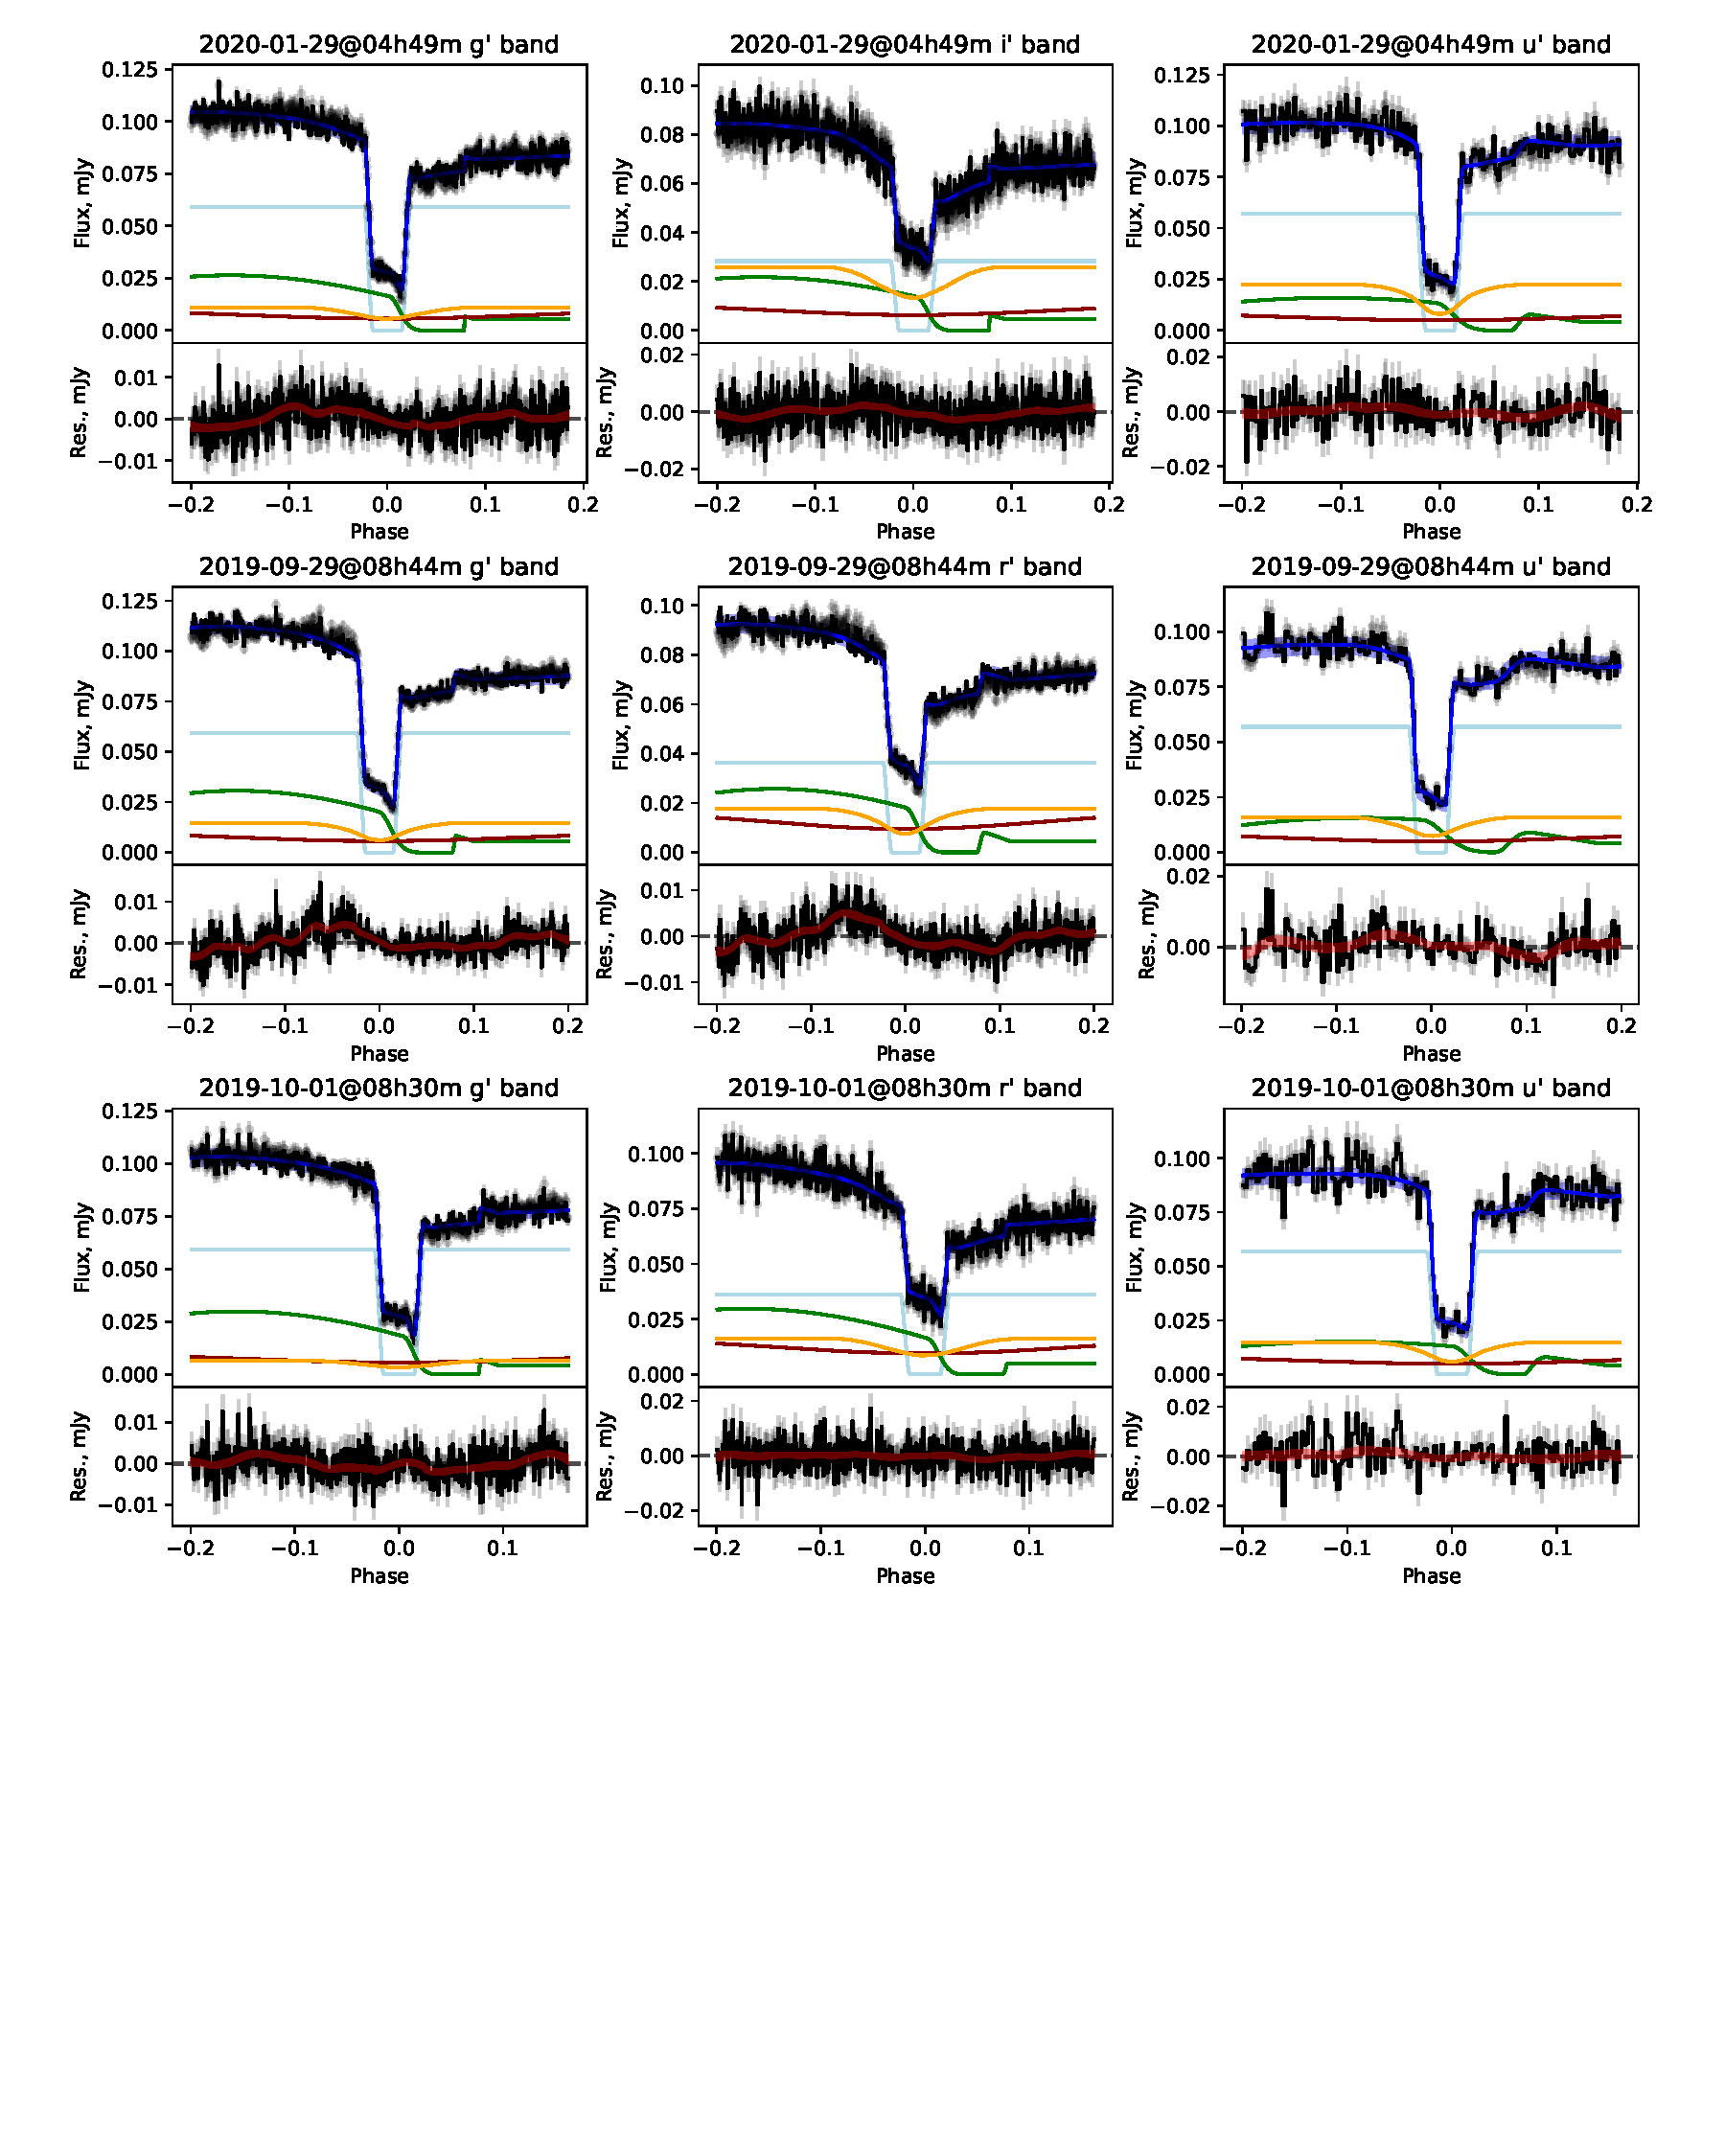
\includegraphics[width=\columnwidth, trim={0cm 10cm 0cm 0cm}, clip]{figures/three_cvs_with_weird_colours/SSS111126/SSS111126_lightcurves_3.pdf}
    \caption{SSSJ0522-3505 lightcurve models. Symbols are the same as Figure \ref{fig:ASASSN-17jf all lightcurves}}
    \label{fig:SSSJ0522-3505 all lightcurves}
\end{figure}


%%%%%%%%%%%%%%%%%%%%%%%%%%%%%%%%%%%%%%%%%%%%%%%%%%